\documentclass[12pt]{article}
\usepackage{amsmath}
\usepackage{amssymb}
\usepackage{geometry}
\usepackage{enumerate}
\usepackage{natbib}
\usepackage{float}%稳定图片位置
\usepackage{graphicx}%画图
\usepackage[english]{babel}
\usepackage{a4wide}
\usepackage{indentfirst}%缩进
\usepackage{enumerate}%加序号
\usepackage{multirow}%合并行


\begin{document}
\newpage
\section{Problem1}
\subsection{(a)}
$$V_{dc}=V_s-V_{on}=5-0.7=4.3(V)$$
$$I_{dc}=\frac{V_{dc}}{R}=\frac{4.3}{5000}=0.86(mA)$$
$$V_r\approx V_{dc}\frac{T}{RC}=4.3\frac{1}{60*5000C}=0.1\rightarrow C\approx143(\mu F)$$
$$\theta_c\approx \sqrt{\frac{2V_r}{V_s}}=\sqrt{\frac{2*0.1}{5}}=0.2(rad)$$
$$\triangle T\approx \frac{\theta_c}{\omega}=\frac{0.2}{2\pi *60}=5.3\times10^{-4}(s)$$
$$I_{surge}=\omega C V_s=2\pi *60*143\times10^{-6}*5=0.27(A)$$
$$I_{peak}=\frac{2I_{dc}T}{\triangle T}=\frac{2*8.6\times10^{-4}}{60*5.3\times10^{-4}}=0.054(A)$$
$$PIV=2V_S-V_{on}=10-0.7=9.3(V)$$
\subsection{(b)}
\begin{figure}[H]
\centering
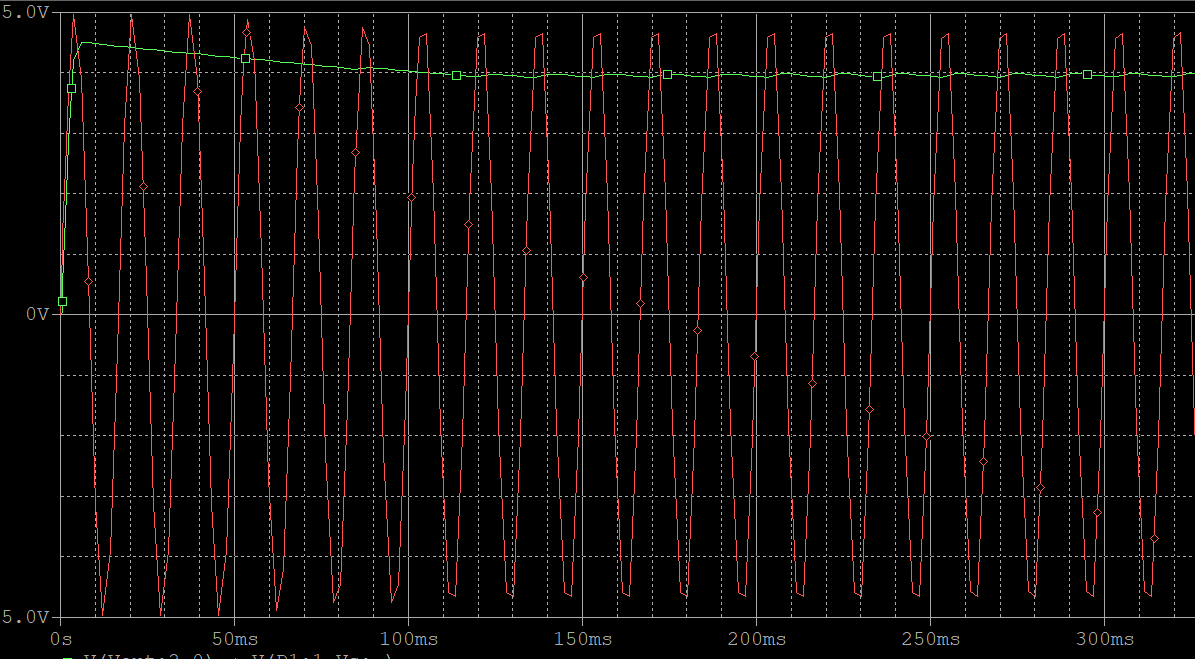
\includegraphics[scale=0.3]{P1.png}
\end{figure}
I can't set the $V_{on}$ for the diode in pspice, but from the graph $V_{dc}=4(V)$, $I_{dc}=0.8(mA)$, $V_r=0.6(V)$ and $PIV=9(V)$. By comparing the simulation result with my calculation result, I find that all simulation results are slightly smaller than the calculation results, but there is not much big difference. I think it's due to the fact that the diode in pspice has a higher $V_{out}=1(V)$ so that $V_{dc}$, $V_{r}$, $I_{dc}$ and $PIV$ are smaller. 
\subsection{(c)}
\begin{figure}[H]
\centering
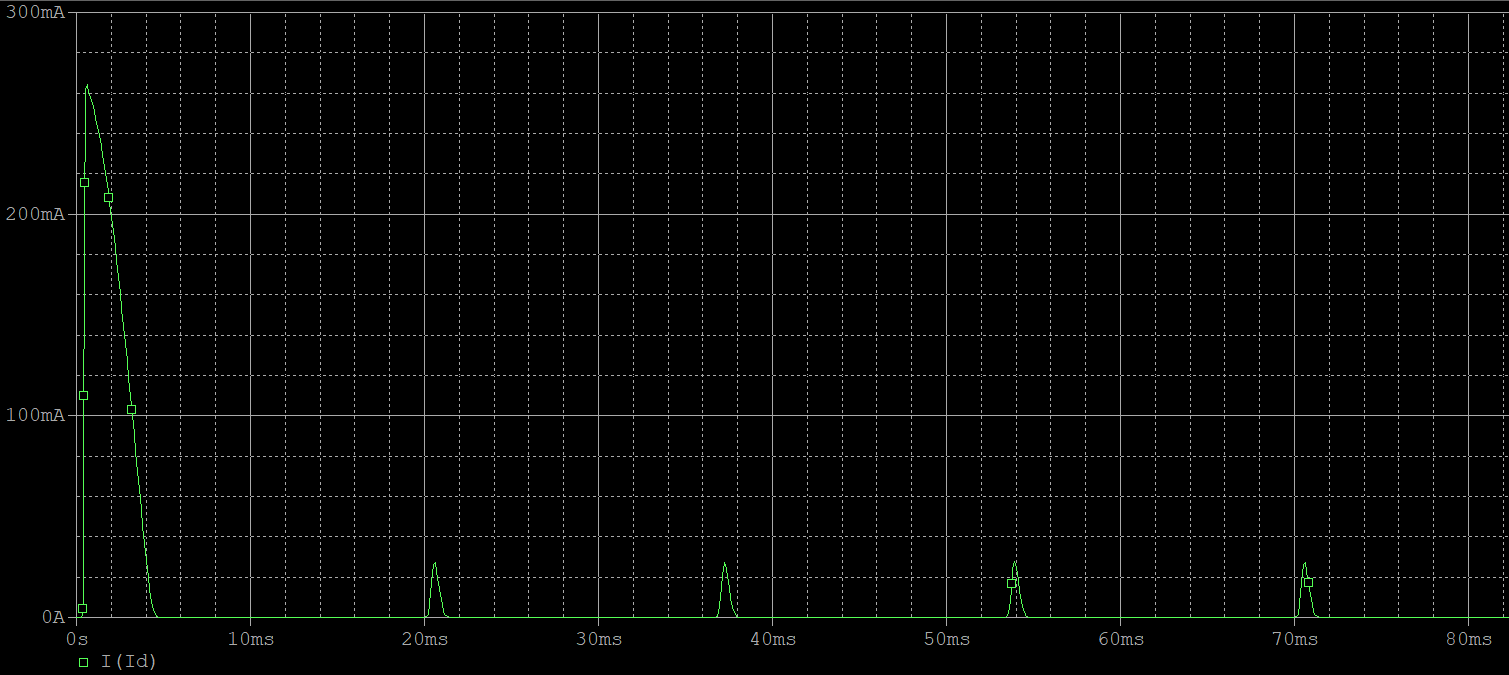
\includegraphics[scale=0.3]{P2.png}
\end{figure}
\par From the simulation and graphs, $I_{surge}\approx 0.26(A)$, and $I_{peak} \approx 26(mA)$ and
$I_{surge}$ is very close to my calculation result but $I_{peak}$ is much smaller, I think this difference is caused by my reading error.

\section{Problem2}
\subsection{(a)}
$$V_{dc}=V_s-2V_{on}=5-2*0.7=3.6(V)$$
$$I_{dc}=\frac{V_{dc}}{R_{dc}}=\frac{3.6}{5000}=0.72(mA)$$
$$V_r\approx V_{dc}\frac{T}{RC}=3.6\frac{1}{2*60*5000C}=0.1\rightarrow C\approx60(\mu F)$$
$$\theta_c\approx \sqrt{\frac{2V_r}{V_s}}=\sqrt{\frac{2*0.1}{5}}=0.2(rad)$$
$$\triangle T\approx \frac{\theta_c}{\omega}=\frac{0.2}{2\pi *60}=5.3\times10^{-4}(s)$$
$$I_{surge}=\omega C V_s=2\pi *60*60\times10^{-6}*5=0.113(A)$$
$$I_{peak}=\frac{I_{dc}T}{\triangle T}=\frac{8.6\times10^{-4}}{60*5.3\times10^{-4}}=0.0225(A)$$
$$PIV=V_S-V_{on}=5-0.7=4.3(V)$$

\subsection{(b)}
\begin{figure}[H]
\centering
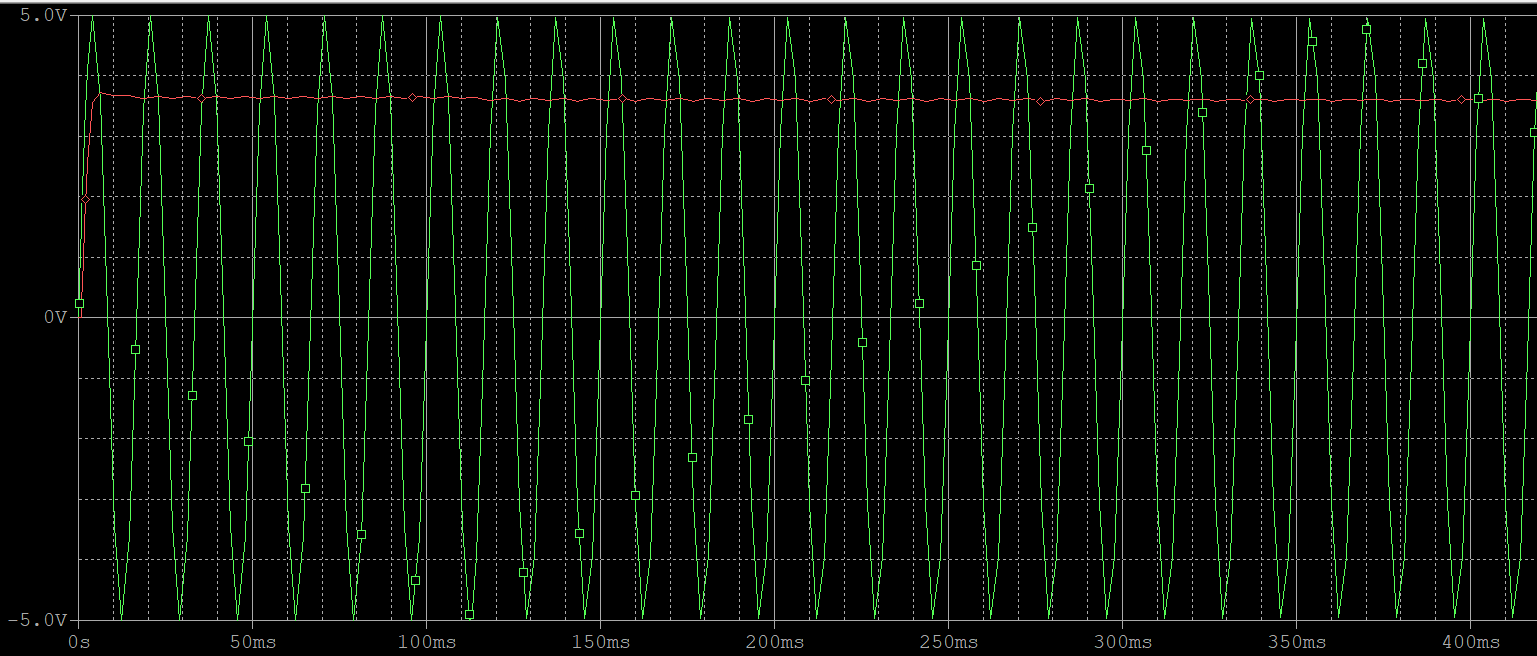
\includegraphics[scale=0.3]{P3.png}
\end{figure}
I can't set the $V_{on}$ for the diode in pspice, but from the graph $V_{dc}=3.6(V)$, $I_{dc}=0.72(mA)$, $V_r=0.02(V)$ and $PIV=4(V)$. By comparing the simulation result with my calculation result, I find that all simulation results are slightly closer to the calculation results than half-wave rectifier, I think it's because there are more diodes so that the difference of $V_{out}$ is reduced
\subsection{(c)}
\begin{figure}[H]
\centering
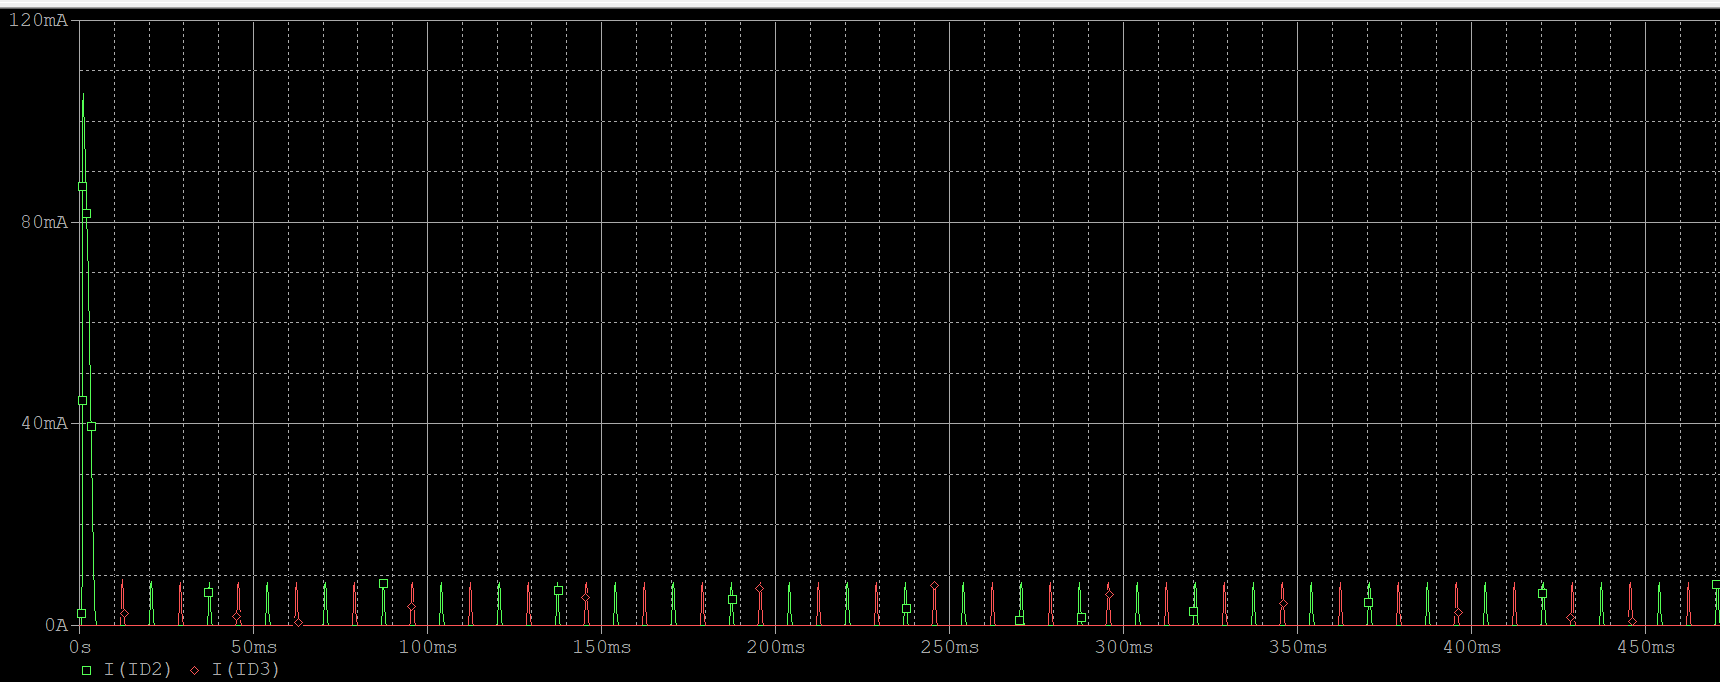
\includegraphics[scale=0.3]{P4.png}
\par From the simulation and graphs, $I_{surge}\approx 0.212(A)$, and $I_{peak} \approx 10(mA)$,
$I_{surge}$ is very close to my calculation result, but $I_{peak}$ is much smaller from calculation results. In addition, only one of these two currents has $I_{surge}$ while their currents both have $I_{peak}$ and they have the same value. When one of these currents is 0, the other is at $I_{peak}$
\end{figure}
\end{document}